\chapter{HerBS SEDs}

\begin{figure}
	\centering
	\caption[SEDs of HerBS sample (Optically thin)]{SEDs of the HerBS sample (optically thin model) and the residuals on the best fitting model. The shaded regions represent the $16$th to $84$th percentiles in the range of SEDs explored during fitting.}
	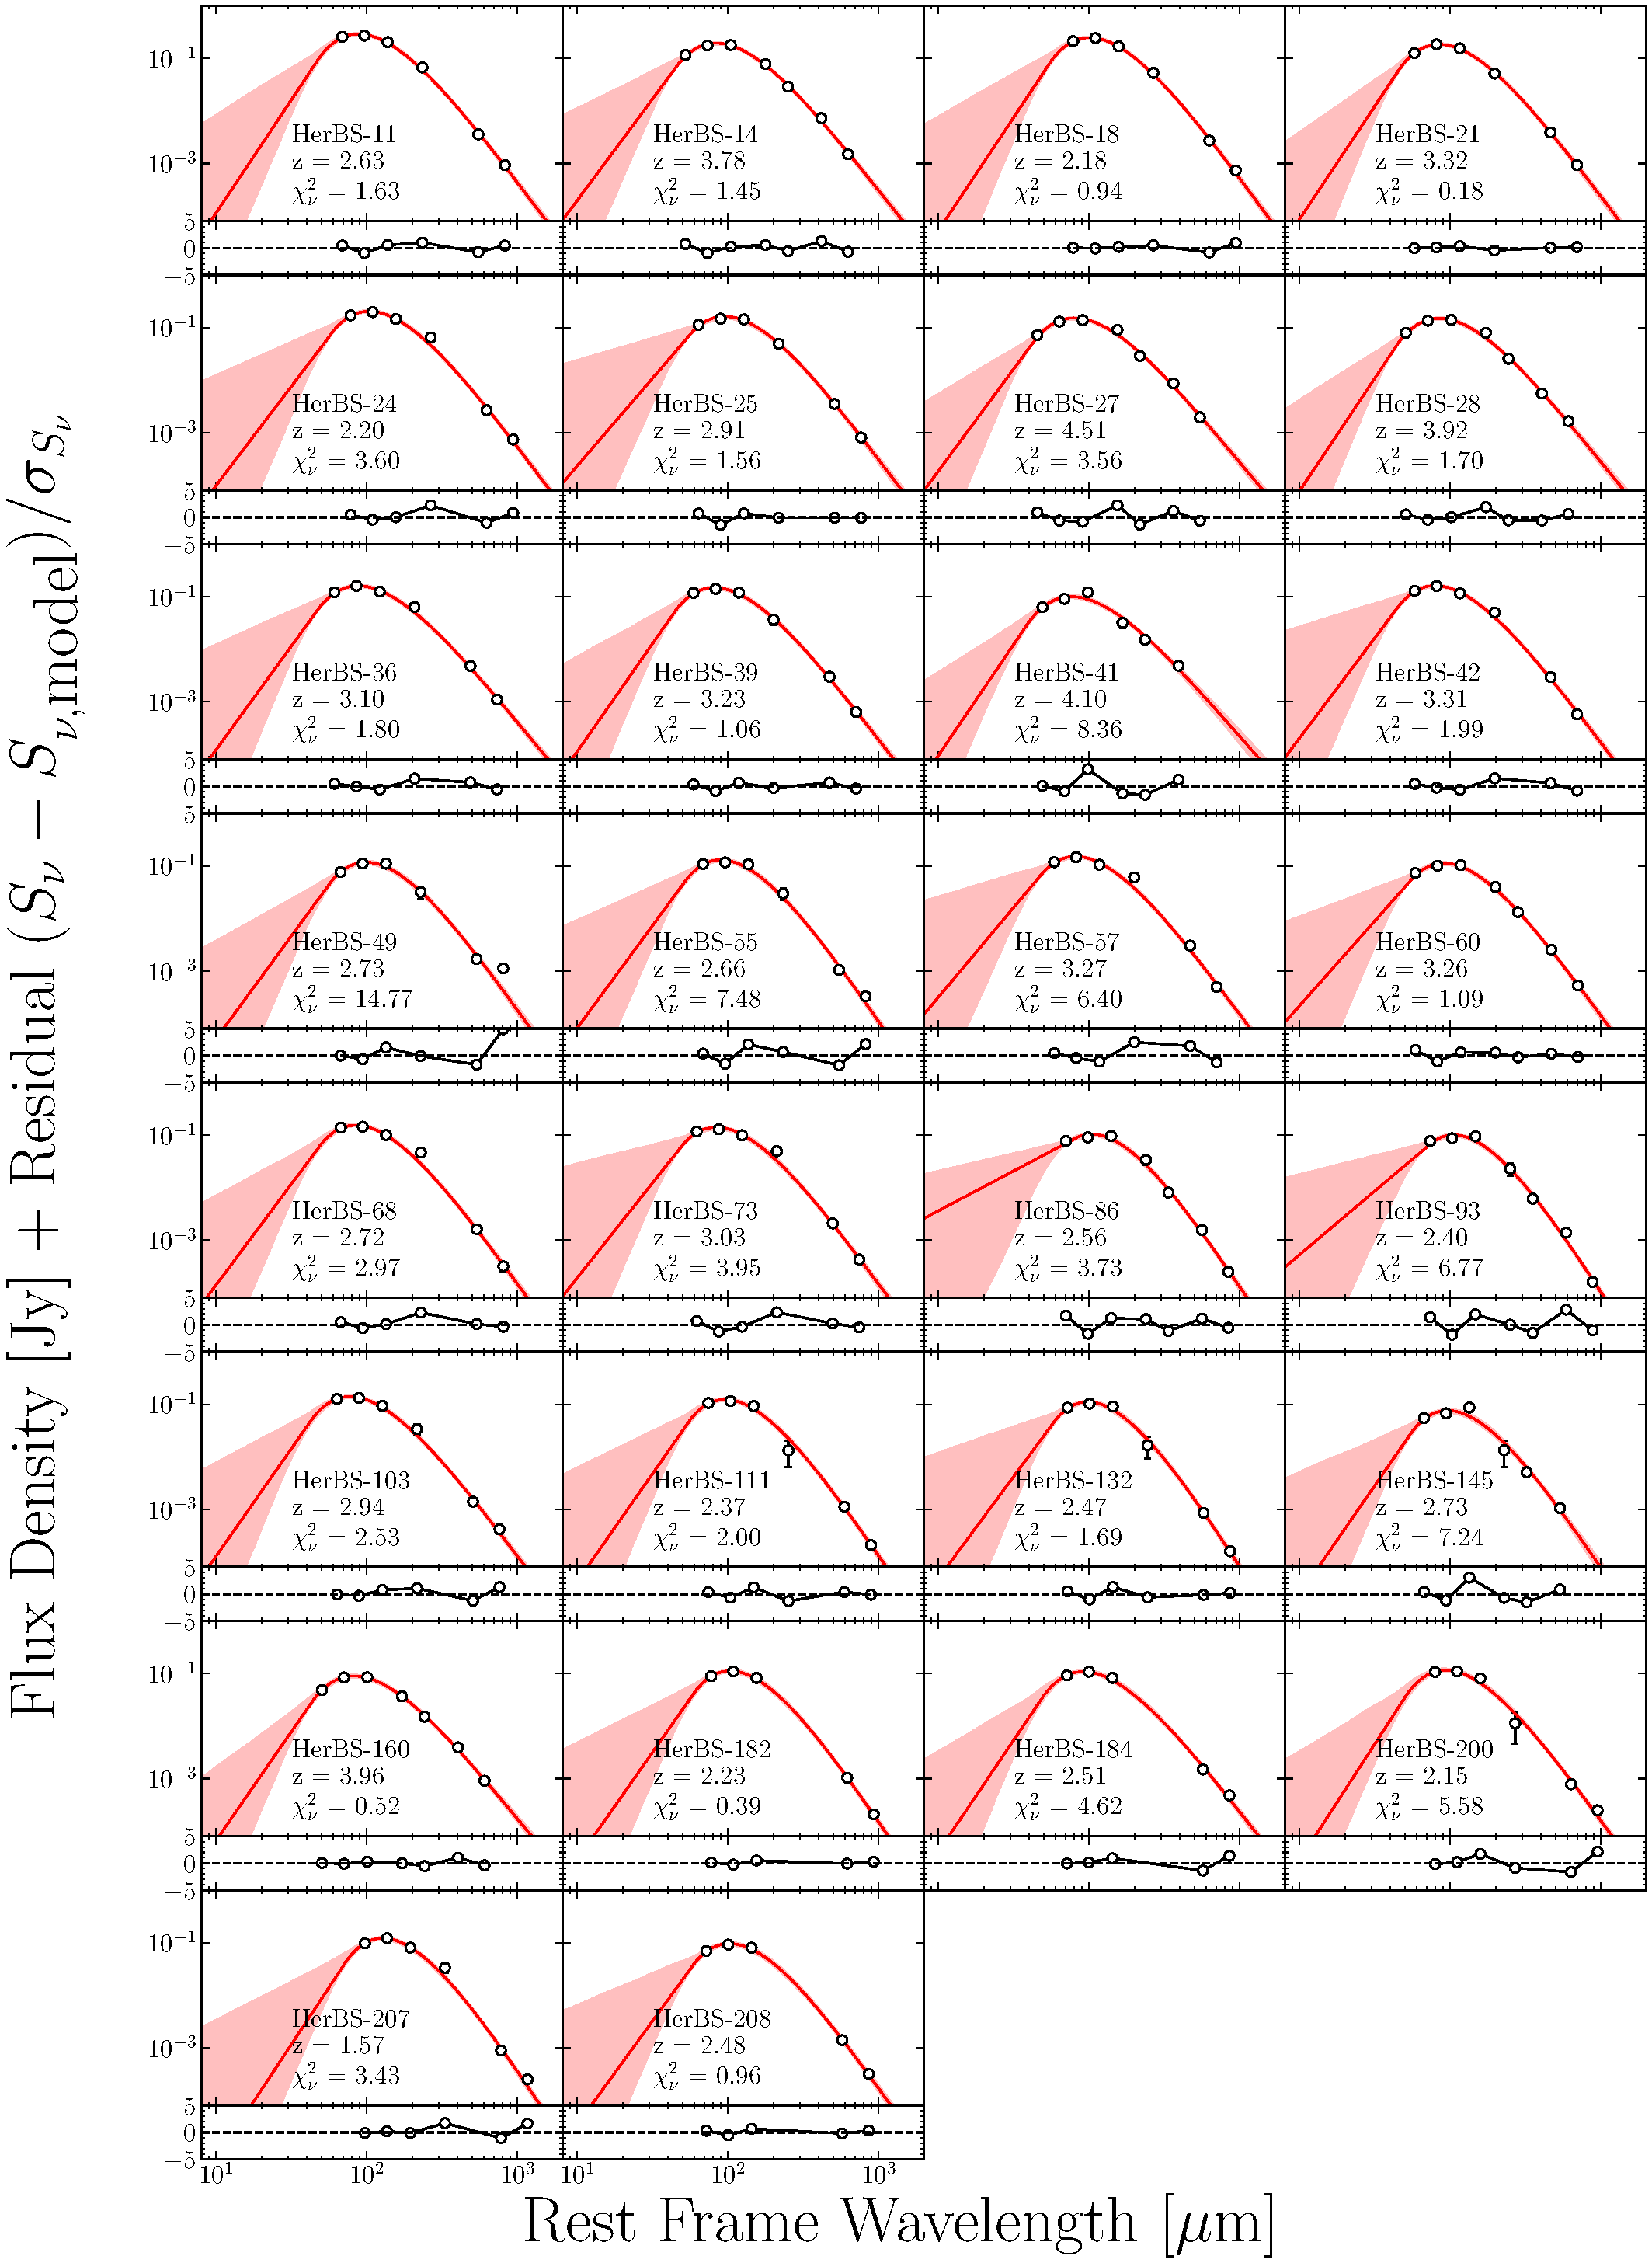
\includegraphics[width=\columnwidth]{Figures/Figure_C_1.pdf}
\end{figure}

\begin{figure}
	\centering
	\caption[SEDs of HerBS sample ($\lambda_1 = 100\,\mu$m)]{SEDs of the HerBS sample ($\lambda_1 = 100\,\mu$m) and the residuals on the best fitting model. The shaded regions represent the $16$th to $84$th percentiles in the range of SEDs explored during fitting.}
	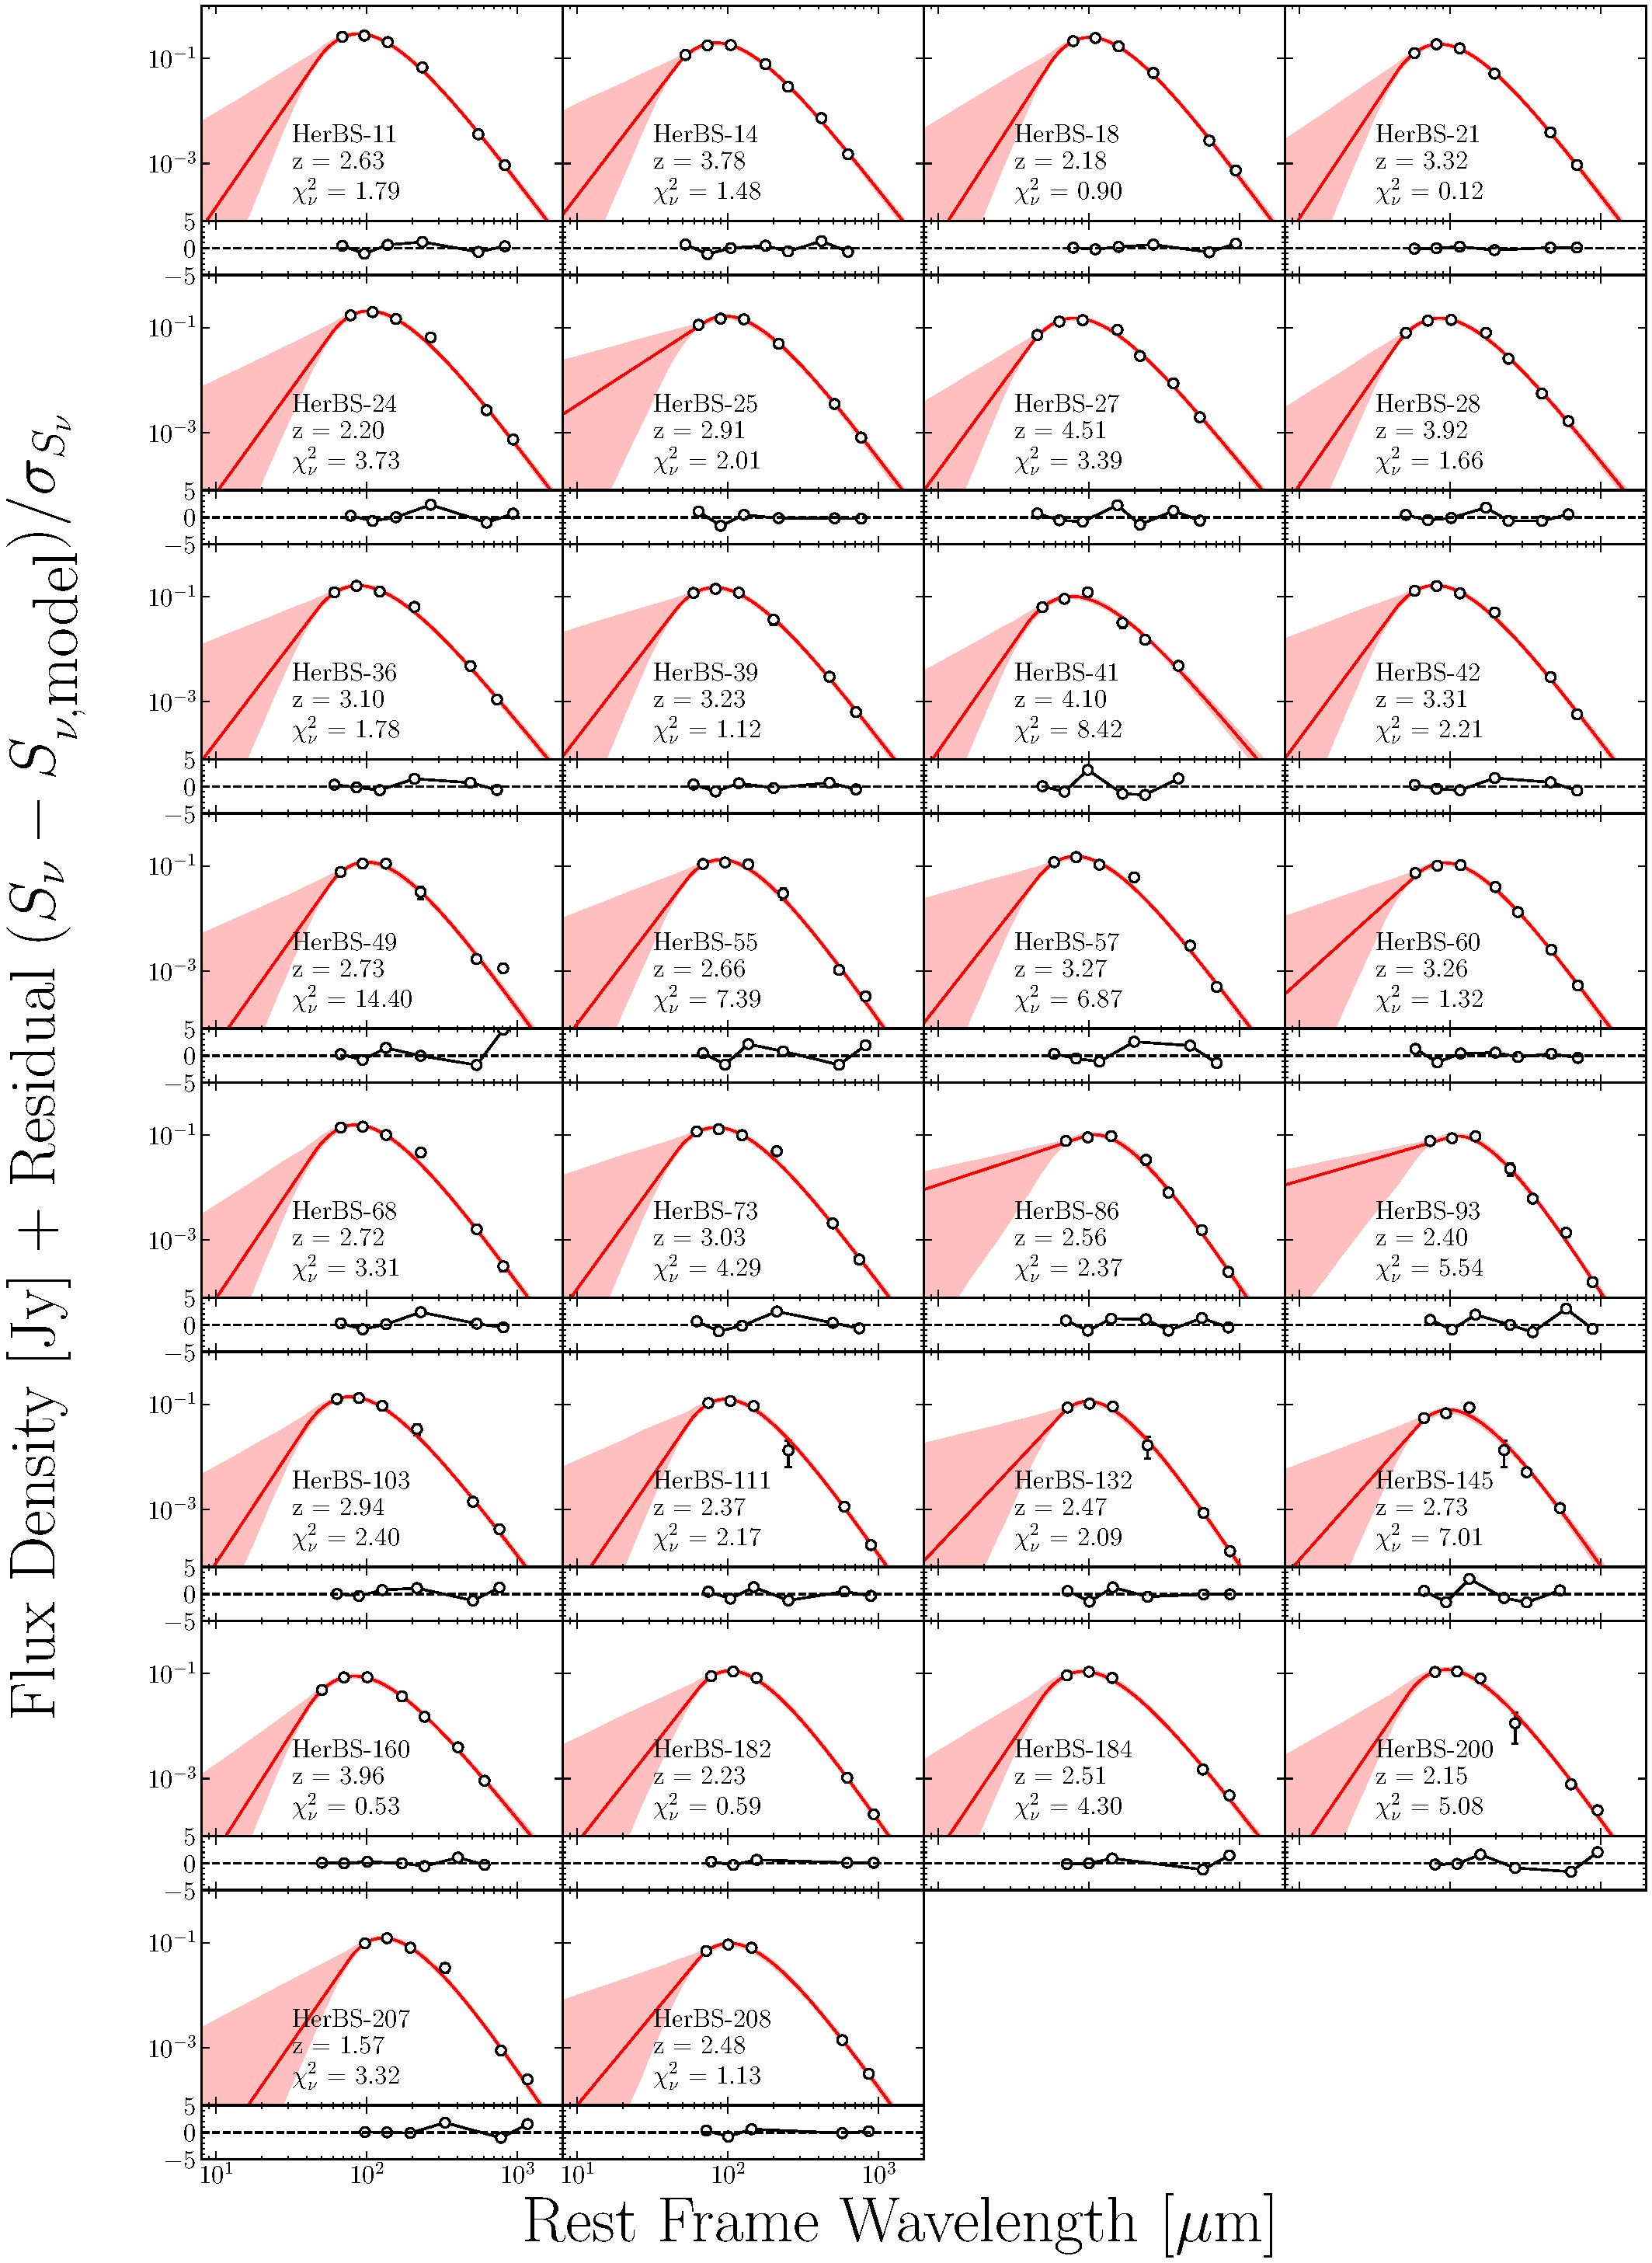
\includegraphics[width=\columnwidth]{Figures/Figure_C_2.pdf}
\end{figure}

\begin{figure}
	\centering
	\caption[SEDs of HerBS sample ($\lambda_1 = 200\,\mu$m)]{SEDs of the HerBS sample ($\lambda_1 = 200\,\mu$m) and the residuals on the best fitting model. The shaded regions represent the $16$th to $84$th percentiles in the range of SEDs explored during fitting.}
	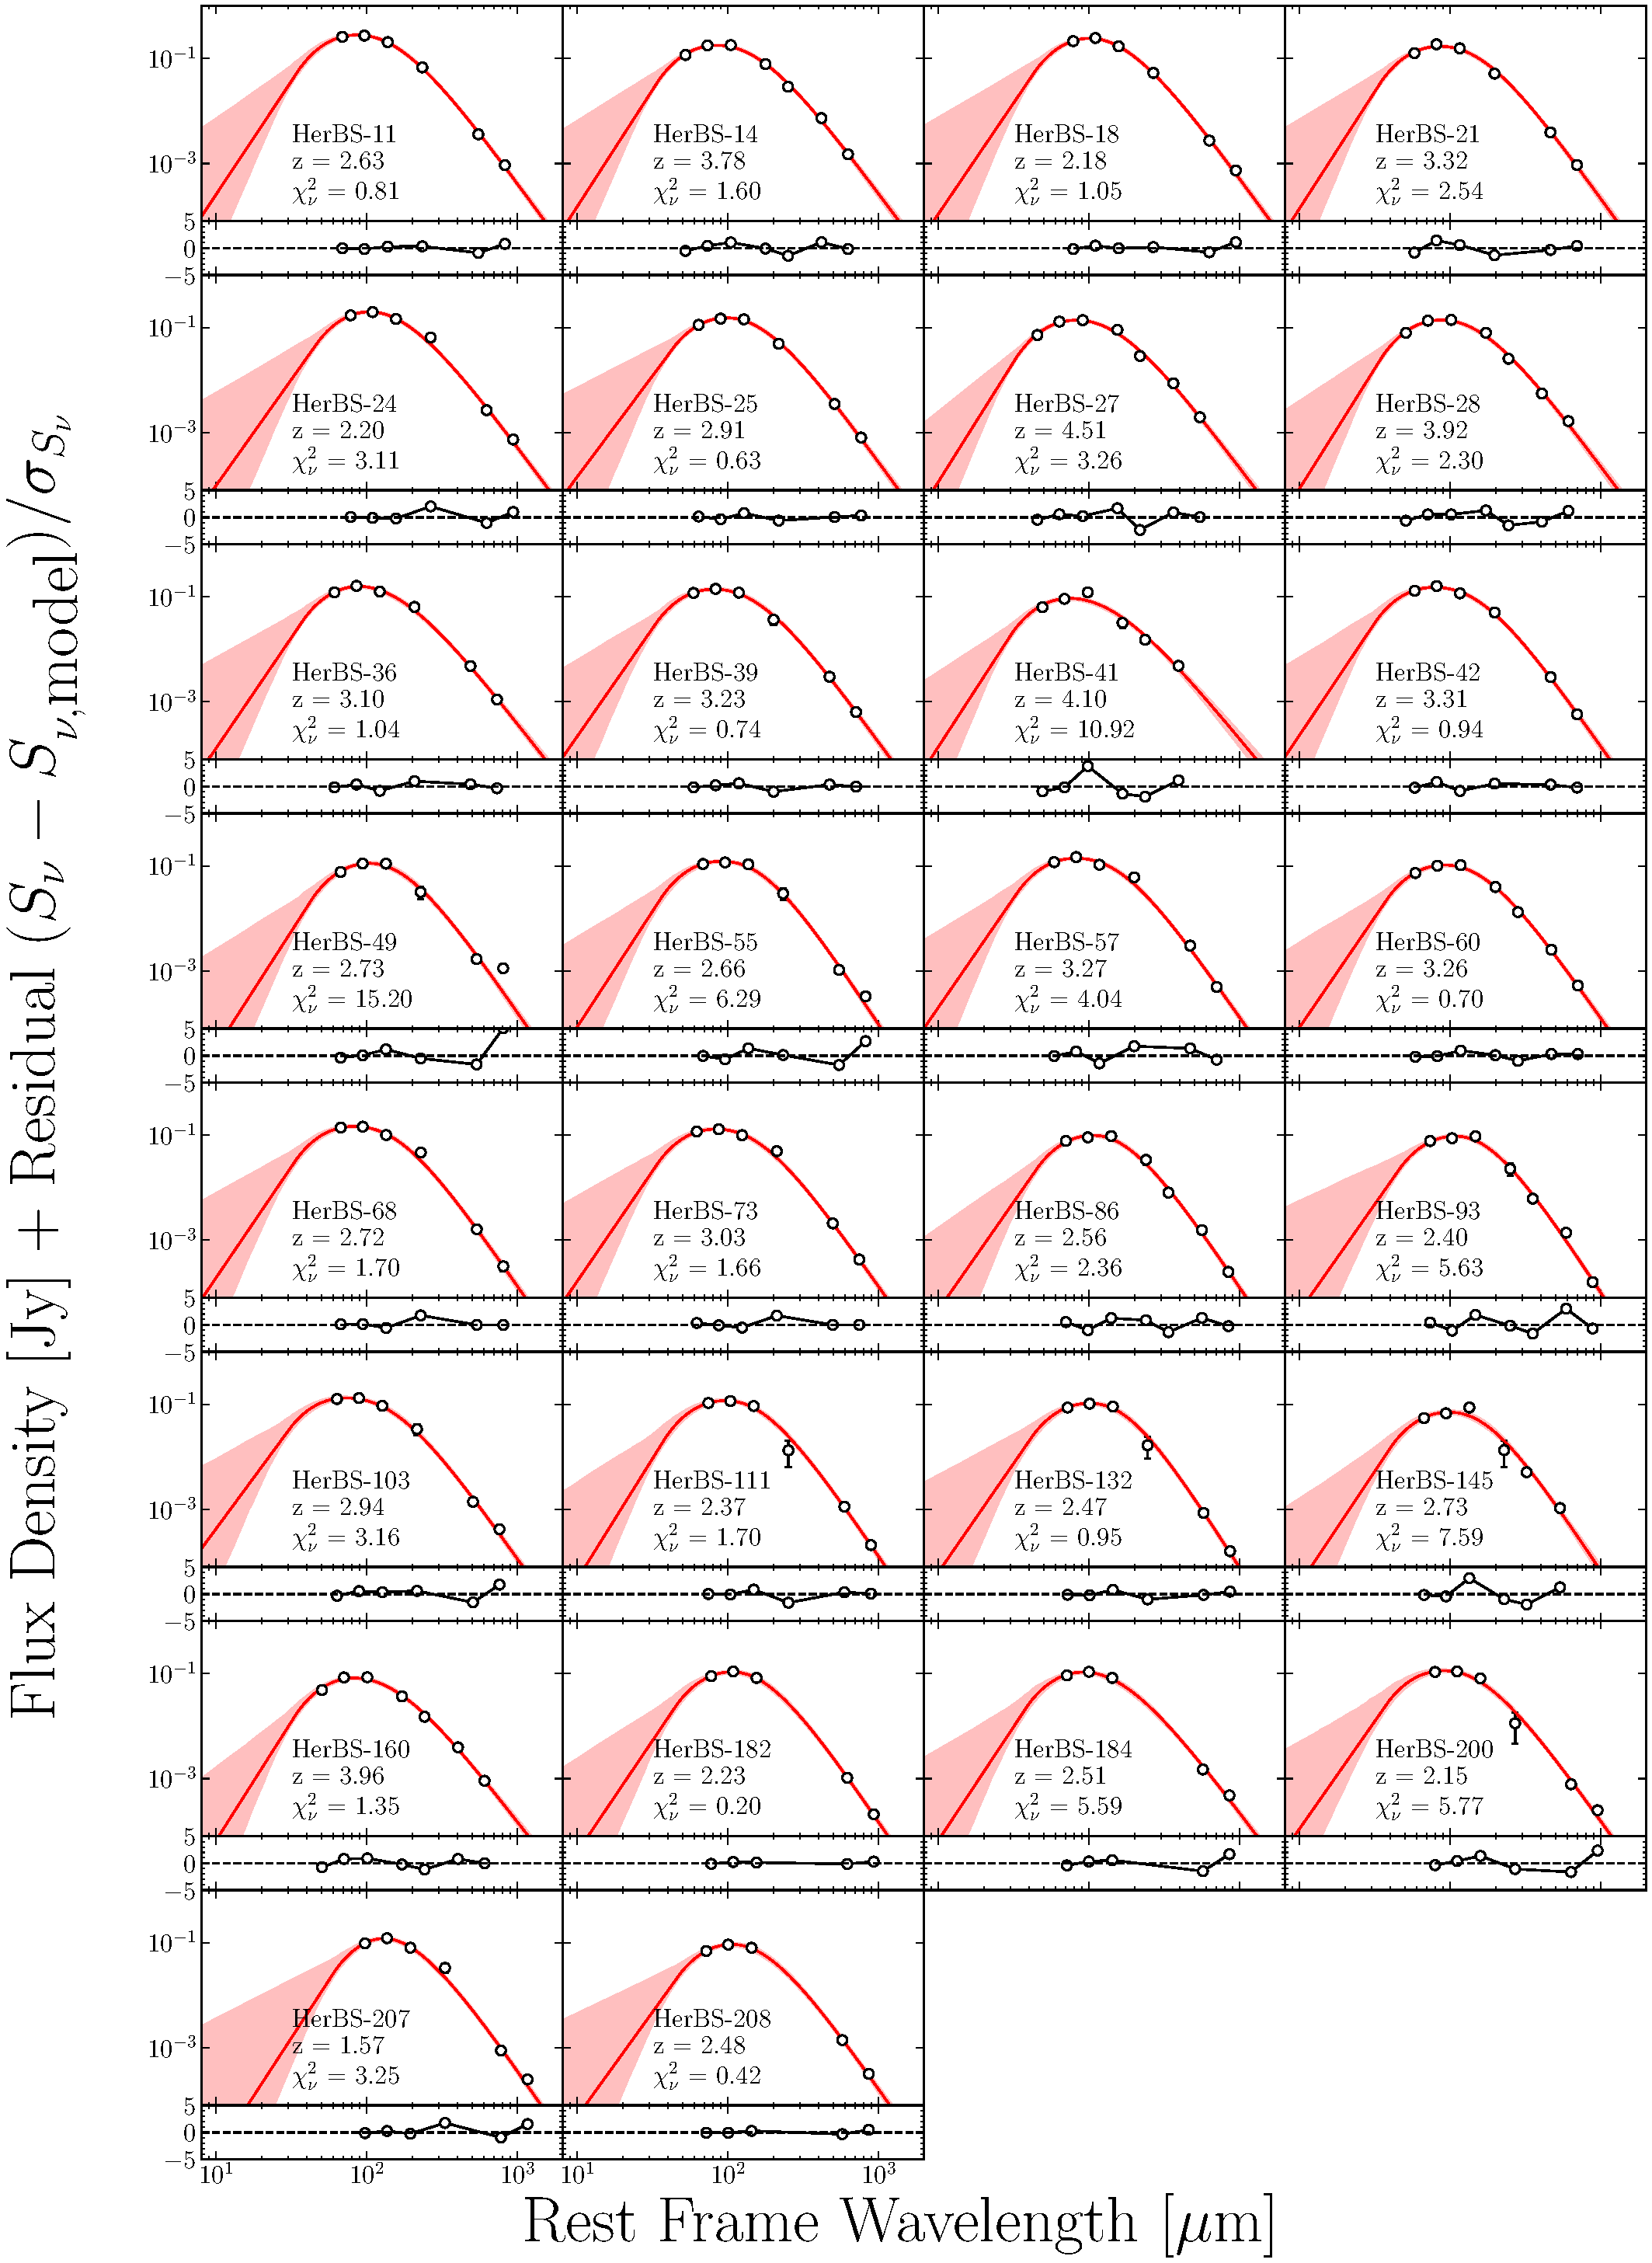
\includegraphics[width=\columnwidth]{Figures/Figure_C_3.pdf}
\end{figure}